\documentclass[a4paper,12pt]{article}

% ---------------- Encoding & Language ----------------
\usepackage[utf8]{inputenc}
\usepackage[T5]{fontenc} % better for Vietnamese diacritics
\usepackage[english,vietnamese]{babel}

% ---------------- Packages ----------------
\usepackage{amsmath,amssymb}
\usepackage{array}
\usepackage{textcomp}
\usepackage{xcolor}
\usepackage{graphicx}
\usepackage{geometry}
\usepackage{float}
\usepackage{mdframed}
\usepackage{nopageno}
\usepackage{fancyhdr}
\usepackage{ulem}
\usepackage{tcolorbox}
\usepackage{tocloft}
\usepackage{hyperref}
\usepackage{subcaption}
\usepackage{listings}
\usepackage{longtable}
\usepackage{booktabs}
\usepackage{tabularx}
\usepackage{adjustbox}

% ---------------- Page setup ----------------
\geometry{a4paper, margin=0.75in}
\setlength{\parindent}{0pt} % remove paragraph indentation so lines start flush left

\mdfdefinestyle{MyFrame}{%
    linecolor=blue,
    outerlinewidth=2pt,
    roundcorner=0pt,
    innertopmargin=10pt,
    innerbottommargin=10pt,
    innerrightmargin=10pt,
    innerleftmargin=10pt,
    backgroundcolor=white
}

% ---------------- Colors for listings ----------------
\definecolor{comment}{RGB}{0,128,0}   % green for comments
\definecolor{kwpink}{RGB}{255,20,147} % pink for keywords
\definecolor{numblue}{RGB}{0,0,200}   % blue for numeric literals
\definecolor{string}{RGB}{163,21,21}  % string color (dark red)
\definecolor{framegray}{RGB}{200,200,200}

% ---------------- Listing configuration ----------------
% ---------------- Listing configuration ----------------
\lstset{
    language=C,                       % use C syntax highlighting
    basicstyle=\ttfamily\small,
    keywordstyle=\color{kwpink}\bfseries, % pink for keywords
    commentstyle=\color{comment}\itshape, % green comments
    stringstyle=\color{string},        % dark red strings
    numbers=left,
    numberstyle=\tiny\color{gray},
    stepnumber=1,
    numbersep=6pt,
    backgroundcolor=\color{white},
    frame=single,
    rulecolor=\color{framegray},
    breaklines=true,
    tabsize=4,
    showspaces=false,
    showstringspaces=false,
    alsoletter={_},
    morekeywords={if,else,while,for,switch,case,return}, % only control-flow pink
    deletekeywords={HAL_Delay}, % make sure HAL_Delay is not colored as keyword
    literate=%
     *{0}{{{\color{numblue}0}}}1
      {1}{{{\color{numblue}1}}}1
      {2}{{{\color{numblue}2}}}1
      {3}{{{\color{numblue}3}}}1
      {4}{{{\color{numblue}4}}}1
      {5}{{{\color{numblue}5}}}1
      {6}{{{\color{numblue}6}}}1
      {7}{{{\color{numblue}7}}}1
      {8}{{{\color{numblue}8}}}1
      {9}{{{\color{numblue}9}}}1
      {.}{{{\color{numblue}.}}}1
}

% ---------------- Header / Footer ----------------
\pagestyle{fancy}
\fancyhf{}
\fancyhead[L]{\small Ho Chi Minh City University of Technology \\ Faculty of Computer Science and Engineering}
\fancyhead[R]{
\includegraphics[height=20pt]{bk_logo.png}}
\fancyfoot[C]{\thepage}
\renewcommand{\headrulewidth}{1.5pt}
\renewcommand{\footrulewidth}{1.5pt}

% ---------------- Document ----------------
\begin{document}
\selectlanguage{vietnamese}

\begin{mdframed}[style=MyFrame]
\thispagestyle{empty}
\begin{center}
    \vspace*{0.5cm}
    {\large \textbf{TRƯỜNG ĐẠI HỌC BÁCH KHOA – TP. HỒ CHÍ MINH}}\\[0.2cm]
    {\large \textbf{KHOA KHOA HỌC VÀ KỸ THUẬT MÁY TÍNH}}\\[0.5cm]
    \textbf{*******************}\\[1cm]

    
\includegraphics[width=0.3\textwidth]{bk_logo.png}\\[2cm]

    {\LARGE \textbf{Lab 1 - LED Animation}}\\[0.5cm]
    {\LARGE \textcolor{blue}{Microcontroller - Microprocessor (Lab)}}\\[0.5cm]
    {\LARGE \textbf{COURSE ID: CO3010 - HK251}}\\[0.5cm]
    \textbf{\large Name: Trương Gia Hy   -   Student ID: 2352458}\\[0.5cm]
    \textbf{\large Supervising Lecturer: Dr. VÕ TUẤN BÌNH}\\[8.5cm]

    {\large TP. Hồ Chí Minh – 2024}
\end{center}
\end{mdframed}

\newpage
\section{Exercise}
The GitHub link for the lab files:
\textcolor{blue}{\url{https://github.com/hygameo/VXL-VDK_2352458}}
\subsection{Exercise 1}
\subsubsection{Report 1: Depict the schematic from Proteus simulation in this report.}
\label{ex1r1}
\begin{figure}[H]
    \centering
    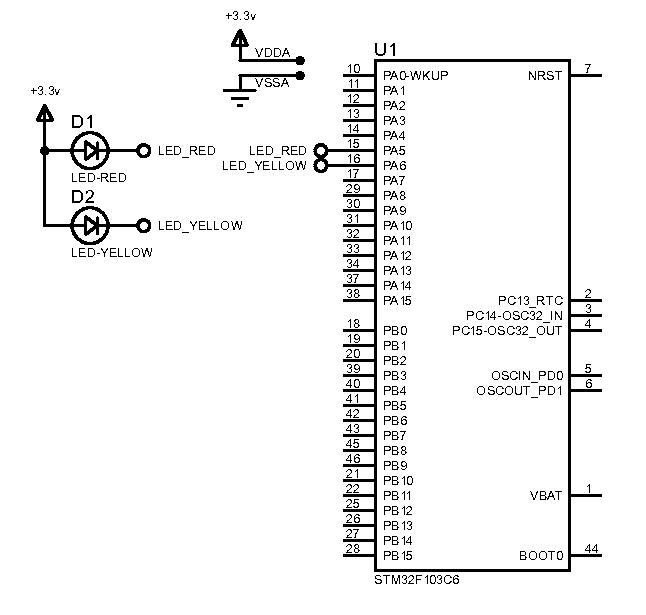
\includegraphics[width=0.95\linewidth]{Attachments/1.1.1.PDF}
\end{figure}
\subsubsection{Report 2: Present the source code in the infinite loop while of your project.}
\begin{lstlisting}
HAL_GPIO_WritePin(GPIOA, LED_RED_Pin, GPIO_PIN_SET);
HAL_GPIO_WritePin(GPIOA, LED_YELLOW_Pin, GPIO_PIN_RESET);

while (1)
{
	HAL_GPIO_TogglePin(GPIOA, LED_RED_Pin | LED_YELLOW_Pin);
	HAL_Delay(2000);
}
\end{lstlisting}
\newpage
\subsection{Exercise 2}
\subsubsection{Report 1: Present the schematic.}
\label{ex2r1}
\begin{figure}[H]
	\centering
	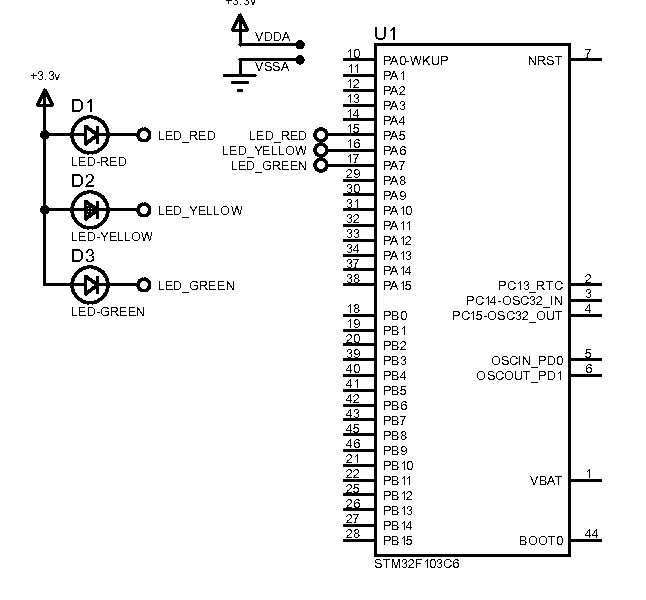
\includegraphics[width=0.95\linewidth]{Attachments/1.2.1.PDF}
\end{figure}
\subsubsection{Report 2: Present the source code in while.}
\begin{lstlisting}
while (1)
{
	HAL_GPIO_WritePin(GPIOA, LED_RED_Pin, GPIO_PIN_RESET);
	HAL_GPIO_WritePin(GPIOA, LED_YELLOW_Pin, GPIO_PIN_SET);
	HAL_GPIO_WritePin(GPIOA, LED_GREEN_Pin, GPIO_PIN_SET);
	HAL_Delay(5000);
	
	HAL_GPIO_TogglePin(GPIOA, LED_RED_Pin | LED_YELLOW_Pin);
	HAL_Delay(2000);
	
	HAL_GPIO_TogglePin(GPIOA, LED_YELLOW_Pin | LED_GREEN_Pin);
	HAL_Delay(3000);
}
\end{lstlisting}
\newpage
\subsection{Exercise 3}
\subsubsection{Report 1: Present the schematic.}
\label{ex3r1}
\begin{figure}[H]
	\centering
	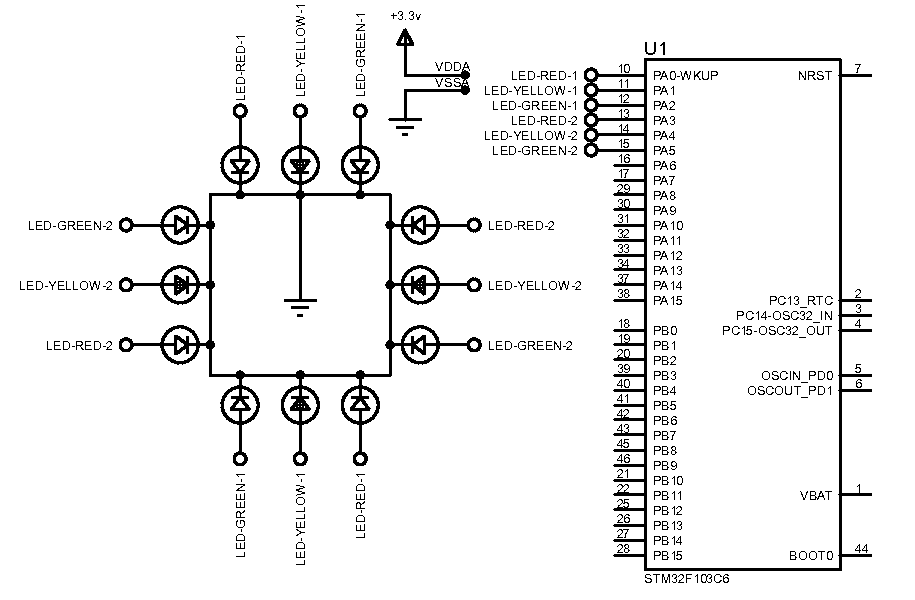
\includegraphics[width=0.95\linewidth]{Attachments/1.3.1.PDF}
\end{figure}
\subsubsection{Report 2: Present the source code in while.}
\begin{lstlisting}
typedef enum {
	RED = 0, YELLOW = 1, GREEN = 2
} LED;
void setLED(LED Road1LED, LED Road2LED, int sec) {
	HAL_GPIO_WritePin(GPIOA,
	LED_RED_1_Pin    | LED_YELLOW_1_Pin |
	LED_GREEN_1_Pin  | LED_RED_2_Pin    |
	LED_YELLOW_2_Pin | LED_GREEN_2_Pin  , GPIO_PIN_RESET);
	HAL_GPIO_TogglePin(GPIOA,
	(Road1LED == RED ? LED_RED_1_Pin : (Road1LED == YELLOW ? LED_YELLOW_1_Pin : LED_GREEN_1_Pin)) |
	(Road2LED == RED ? LED_RED_2_Pin : (Road2LED == YELLOW ? LED_YELLOW_2_Pin : LED_GREEN_2_Pin))
	);
	HAL_Delay(sec * 1000);
}
int main(void){
	while (1){
		setLED(RED, GREEN, 3);
		setLED(RED, YELLOW, 2);
		setLED(GREEN, RED, 3);
		setLED(YELLOW, RED, 2);
	}
}
\end{lstlisting}
\newpage
\subsection{Exercise 4}
\subsubsection{Report 1: Present the schematic.}
\label{ex4r1}
\begin{figure}[H]
	\centering
	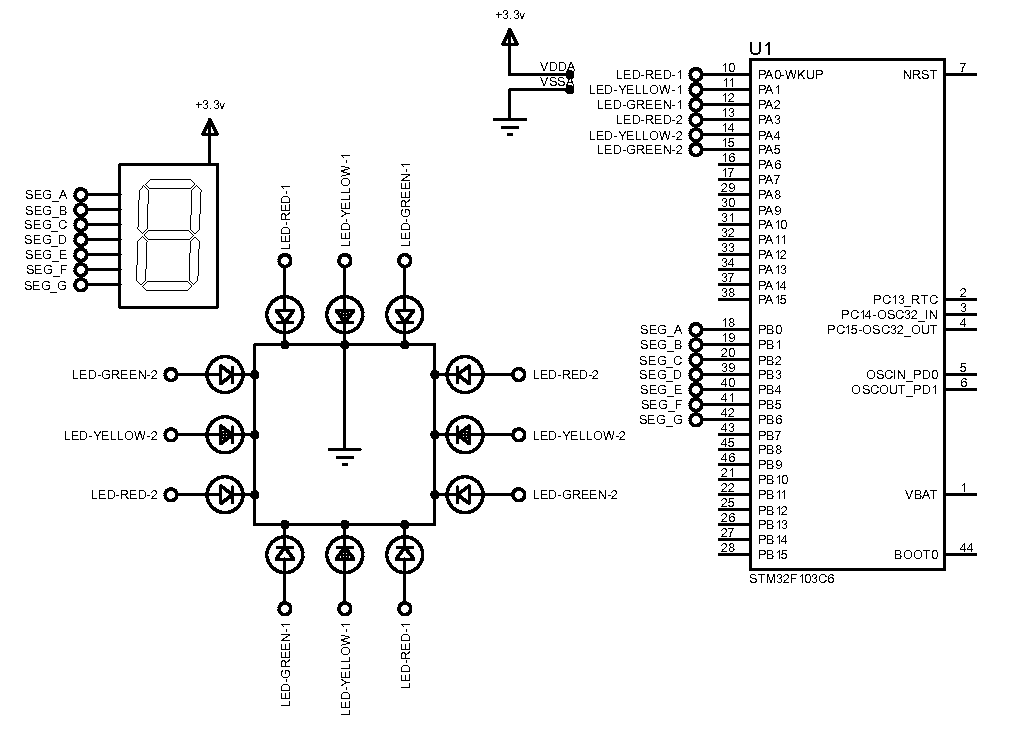
\includegraphics[width=0.95\linewidth]{Attachments/1.4.1.PDF}
\end{figure}
\subsubsection{Report 2: Present the source code for display7SEG function.}
\begin{lstlisting}
uint8_t segmentMap[10] = {
	0b1111110, 0b0110000,
	0b1101101, 0b1111001,
	0b0110011, 0b1011011,
	0b1011111, 0b1110000,
	0b1111111, 0b1111011
};

uint8_t SegPin[7] = {
	SEG_A_Pin, SEG_B_Pin,
	SEG_C_Pin, SEG_D_Pin,
	SEG_E_Pin, SEG_F_Pin,
	SEG_G_Pin
};

void display7SEG(int num) {
	uint8_t bitmask = segmentMap[num];
	
	for(int i = 0; i < 7; i++) HAL_GPIO_WritePin(GPIOB, SegPin[i], (bitmask & (1 << (6 - i))) ? RESET : SET);
}
\end{lstlisting}
\newpage
\subsection{Exercise 5}
\subsubsection{Report 1: Present the source code.}
\begin{lstlisting}
typedef enum {
	RED = 0, YELLOW = 1, GREEN = 2
} LED;
uint8_t segmentMap[10] = {
	0b1111110, 0b0110000,
	0b1101101, 0b1111001,
	0b0110011, 0b1011011,
	0b1011111, 0b1110000,
	0b1111111, 0b1111011
};
uint8_t SegPin[7] = {
	SEG_A_Pin, SEG_B_Pin,
	SEG_C_Pin, SEG_D_Pin,
	SEG_E_Pin, SEG_F_Pin,
	SEG_G_Pin
};
void display7SEG(int num) {
	uint8_t bitmask = segmentMap[num];
	
	for(int i = 0; i < 7; i++) HAL_GPIO_WritePin(GPIOB, SegPin[i], (bitmask & (1 << (6 - i))) ? RESET : SET);
}
void setLED(LED Road1LED, LED Road2LED, int sec){
	HAL_GPIO_WritePin(GPIOA,
	LED_RED_1_Pin    | LED_YELLOW_1_Pin |
	LED_GREEN_1_Pin  | LED_RED_2_Pin    |
	LED_YELLOW_2_Pin | LED_GREEN_2_Pin  , GPIO_PIN_RESET);
	
	HAL_GPIO_TogglePin(GPIOA,
	(Road1LED == RED ? LED_RED_1_Pin : (Road1LED == YELLOW ? LED_YELLOW_1_Pin : LED_GREEN_1_Pin)) |
	(Road2LED == RED ? LED_RED_2_Pin : (Road2LED == YELLOW ? LED_YELLOW_2_Pin : LED_GREEN_2_Pin))
	);
	
	for(int i = sec; i > 0; i--){
		display7SEG(i);
		HAL_Delay(1000);
	}
}
int main(void)
{
	while (1)
	{
		setLED(RED, GREEN, 3);
		setLED(RED, YELLOW, 2);
		setLED(GREEN, RED, 3);
		setLED(YELLOW, RED, 2);
	}
}
\end{lstlisting}
\newpage
\subsection{Exercise 6}
\subsubsection{Report 1: Present the schematic.}
\label{ex6r1}
\begin{figure}[H]
	\centering
	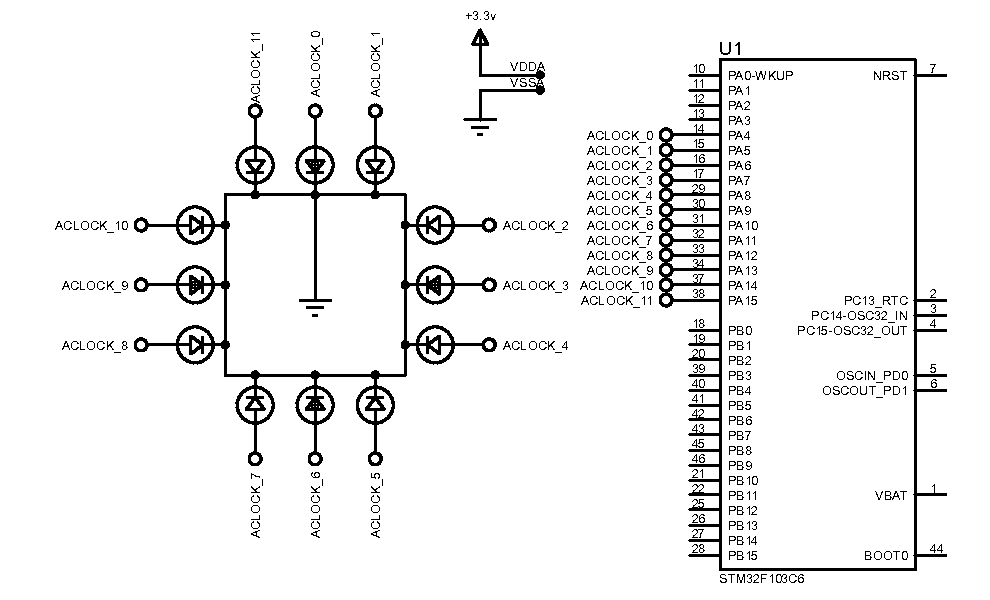
\includegraphics[width=0.95\linewidth]{Attachments/1.6.1.PDF}
\end{figure}
\subsubsection{Report 2: Implement a simple program to test the connection of every single LED. }
\begin{lstlisting}
uint16_t ACLOCK_Pins[12] = {
	ACLOCK_0_Pin , ACLOCK_1_Pin , ACLOCK_2_Pin ,
	ACLOCK_3_Pin , ACLOCK_4_Pin , ACLOCK_5_Pin ,
	ACLOCK_6_Pin , ACLOCK_7_Pin , ACLOCK_8_Pin ,
	ACLOCK_9_Pin , ACLOCK_10_Pin, ACLOCK_11_Pin
};

int main(void)
{
	while (1)
	{
		for(int i = 0; i < 12; i++){
			HAL_GPIO_WritePin(GPIOA, ACLOCK_Pins[i], GPIO_PIN_SET);
			HAL_Delay(250);
		}
		for(int i = 11; i > 0; i--){
			HAL_GPIO_WritePin(GPIOA, ACLOCK_Pins[i], GPIO_PIN_RESET);
			HAL_Delay(250);
		}
	}
}
\end{lstlisting}
\newpage
\subsection{Exercise 7}
\subsubsection{Report 1: Present the source code of this function.}
\begin{lstlisting}
void clearAllClock(void) {
	for (int i = 0; i < 12; i++) HAL_GPIO_WritePin(GPIOA, ACLOCK_Pins[i], GPIO_PIN_RESET);
}
\end{lstlisting}
\subsection{Exercise 8}
\subsubsection{Report 1: Present the source code of this function.}
\begin{lstlisting}
void setNumberOnClock(int num) {
	HAL_GPIO_WritePin(GPIOA, ACLOCK_Pins[num], GPIO_PIN_SET);
}
\end{lstlisting}
\subsection{Exercise 9}
\subsubsection{Report 1: Present the source code of this function.}
\begin{lstlisting}
void clearNumberOnClock(int num) {
	HAL_GPIO_WritePin(GPIOA, ACLOCK_Pins[num], GPIO_PIN_RESET);
}
\end{lstlisting}
\subsection{Exercise 10}
\subsubsection{Report 1: Integrate the whole system and use 12 LEDs to display a clock.}
\begin{lstlisting}
int hour = 0;
int minute = 0;
int second = 0;

while (1)
{
	clearAllClock();
	setNumberOnClock(hour % 12);
	setNumberOnClock((minute / 5) % 12);
	setNumberOnClock((second / 5) % 12);
	
	second++;
	
	if(second == 60){ second = 0; minute++; }
	if(minute == 60){ minute = 0; hour++; }
	
	if(hour == 12) hour = 0;
	
	HAL_Delay(10);
}
\end{lstlisting}
\end{document}


